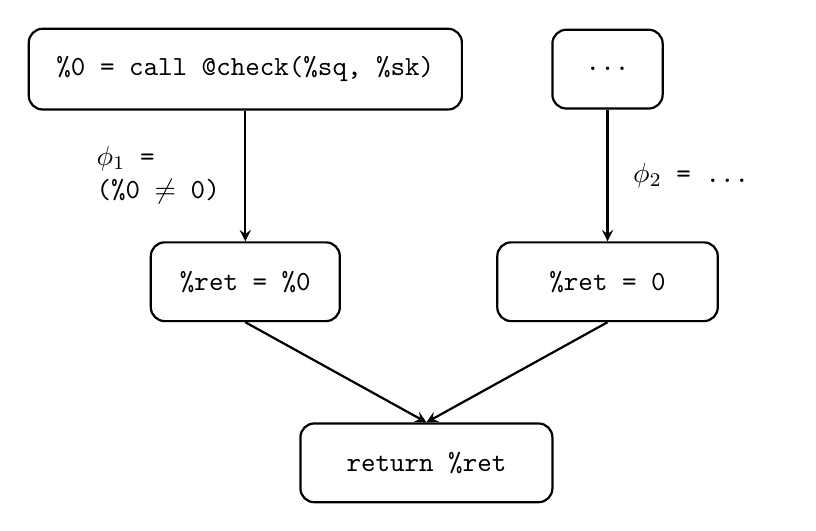
\begin{tikzpicture}[
    bb/.style={
        rectangle,
        rounded corners=5pt,
        draw=black,
        thick,
        minimum height=1cm,
        minimum width=2.8cm,
        inner sep=10pt,
        font=\ttfamily\normalsize,
        align=center
    },
    edge_label/.style={
        font=\ttfamily\normalsize,
        midway
    },
    >=stealth
]

    % 顶层节点 (Top level)
    \node[bb] (check) at (-1.8, 3.2) {\%0 = call @check(\%sq, \%sk)};
    \node[bb, minimum width=1.4cm] (dots) at (2.8, 3.2) {...};

    % 中层节点 (拆分后的赋值节点)
    \node[bb, minimum width=2.4cm] (ve) at (-1.8, 0.5) {\%ret = \%0};
    \node[bb, minimum width=2.8cm] (vok) at (2.8, 0.5) {\%ret = \textbf{0}};

    % 底层返回节点 (Bottom level)
    \node[bb, minimum width=3.2cm] (ret) at (0.5, -1.8) {\textbf{return} \%ret};

    % 连线
    \draw[->, thick] (check.south) -- (ve.north);
    \draw[->, thick] (dots.south) -- (vok.north);
    \draw[->, thick] (ve.south) -- (ret.north);
    \draw[->, thick] (vok.south) -- (ret.north);

    % 条件分支文本标签 (放在箭头左侧)
    \node[font=\ttfamily\normalsize, align=left, anchor=east] at (-2.0, 1.85) {
        $\phi_1$ = \\
        (\%0 $\neq$ \textbf{0})
    };
    \node[font=\ttfamily\normalsize, align=left, anchor=west] at (3.0, 1.85) {
        $\phi_2$ = ...
    };

\end{tikzpicture}